
\chapter{Hierarchical mesh refinement with local time step}
\label{mesh_refinement}



Es conocido que, en problemas transitorios, mantener un paso de tiempo moderado es necesario para obtener una buena solución, mientras que un paso de tiempo excesivo conlleva soluciones muy difusivas. Por otro lado, en dominios grandes suele ser necesario refinar la malla cerca del área de inerés. Este refinado de malla, impone una reducción del paso de tiempo con tal de mantener un número de Courant adecuado. Como resultado, un pequeña región del dominio de cálculo estará imponiendo el paso de tiempo, muy inferior a lo requerido en la mayor parte de éste. Lo que se busca en esta sección es avanzar con un paso de tiempo local en cada subdominio.

La estrategia consiste en un remallado jerárquico, donde cada nivel tiene un tamaño de malla y un paso de tiempo característico. De este modo, cada subdominio avanza con su paso de tiempo propio y se sincroniza con el dominio superior una vez que alcanza el paso de tiempo superior. Al final de este proceso, se toma la solución procedente de la malla más fina.

Este modo de trabajar con un remallado jerárquico facilita mucho la tarea de des-refinado, pues simplemente hay que eliminar elementos del nivel inferior, sin tener que reconstruir conectividades. El principal inconveniente del remallado jerárquico es el tratamiento de los nodos colgantes que aparecen en la frontera de los subdominios. De modo análogo a la discretización espacial, en la discretización temporal también aparecen pasos colgados, que se tienen que interpolar entre dos pasos de tiempo superiores.


\begin{figure}
\centering
\begin{subfigure}{.8\textwidth}
    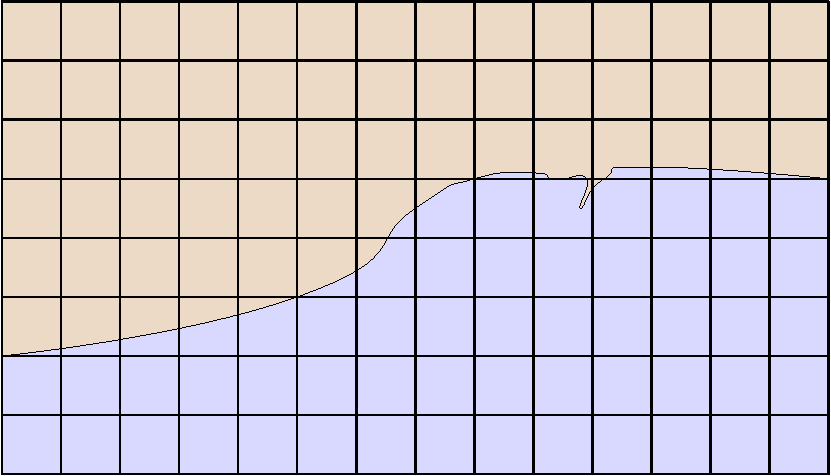
\includegraphics[width=\textwidth]{img/multigrid/grid1.pdf}
    \vspace{1em}
\end{subfigure}
\begin{subfigure}{.8\textwidth}
    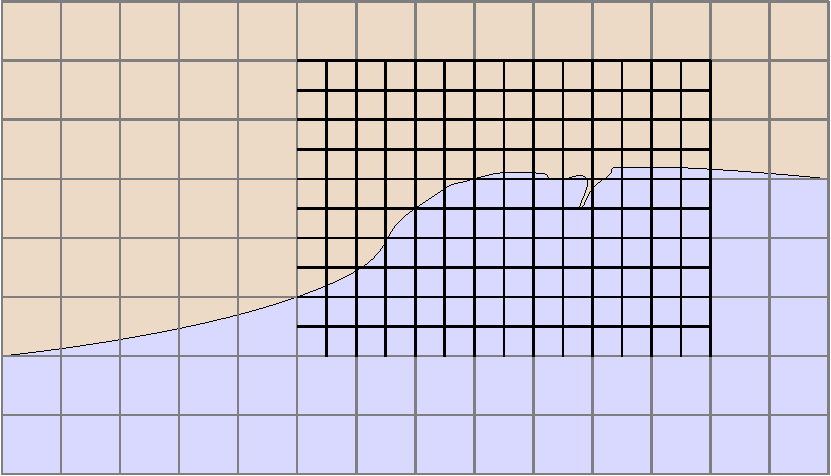
\includegraphics[width=\textwidth]{img/multigrid/grid2.pdf}
    \vspace{1em}
\end{subfigure}
\begin{subfigure}{.8\textwidth}
    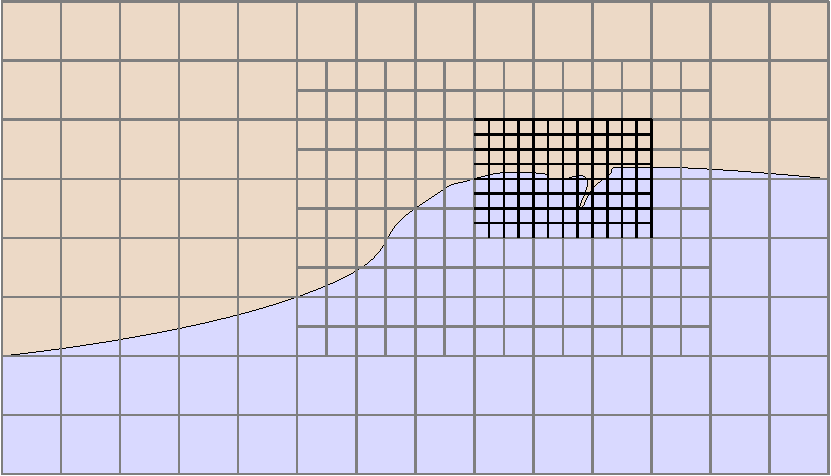
\includegraphics[width=\textwidth]{img/multigrid/grid3.pdf}
    \vspace{1em}
\end{subfigure}
\caption{Different refinement zones for a domain.}
\end{figure}

\section{Algorithm}


\section{Data structure}


\section{Refinement criterion}


\section{Examples}



